\documentclass[sigconf,anonymous,review]{acmart}

% DAI 2026 Research Track permits the ACM sigconf format.  This review draft
% intentionally contains no author-identifying information.
\setcopyright{none}
\settopmatter{printacmref=false,printfolios=true}
\renewcommand\footnotetextcopyrightpermission[1]{}
\pagestyle{plain}

% Additional packages used by this draft.  All are standard TeX Live / Overleaf
% packages; acmart already provides graphicx, booktabs, amsmath, and hyperref.
\usepackage{seqsplit}      % break long SHA-256 digests across lines
\usepackage{algorithm}     % float environment for the CARR decision procedure
\usepackage{algpseudocode} % algorithmicx pseudocode layer

\newcommand{\carr}{\textsc{CARR}}
\newcommand{\norecall}{\textsc{CARR-NoRecall}}
\newcommand{\bbootstrap}{\textsc{Bootstrap}}
\newcommand{\exactfour}{\textsc{Exact-G4}}
\newcommand{\exactfive}{\textsc{Exact-G5}}
\newcommand{\randomfive}{\textsc{Random-G5}}
\newcommand{\jsfive}{\textsc{JS-G5}}
\newcommand{\exactdense}{\textsc{Exact-B25}}

\graphicspath{{../output/pdf/}}

\begin{document}

\title{When Should Global Guidance Be Refreshed? A Paired Pareto Study in Lifelong Multi-Agent Path Finding}

\author{Anonymous Author(s)}

\begin{abstract}
Lifelong multi-agent path finding (LMAPF) requires robot fleets to serve an
ongoing stream of goals while avoiding congestion. Learned global guidance can
improve traffic flow, but existing online methods commonly refresh guidance at
fixed intervals. Frequent refresh consumes generator calls even when demand is
stable, whereas infrequent refresh may leave guidance stale after workload
shifts. We formulate refresh timing as a budgeted control problem and
introduce Context-Aware Refresh and Recall (\carr), which causally chooses to
retain active guidance, generate a new graph, or reactivate a previously
generated one using demand change, context similarity, guidance age, and
route-adoption signals. \carr wraps a frozen generator and planner without
retraining either. We evaluate eight refresh policies on stationary and
non-stationary warehouse workloads using
paired, policy-independent task streams and an audit-complete protocol.
The pre-specified primary objective is not met: dense refresh retains a small
but measurable mean-throughput advantage (\carr effect $-0.80\%$; 95\% CI
$[-1.19\%,-0.40\%]$), so 1\% non-inferiority is not established. In
pre-specified secondary analyses, \carr uses about 79\% fewer generator calls,
forms a non-dominated sample-mean throughput--call operating point, and
significantly outperforms all five evaluated low-call comparators. Our results
identify guidance timing as an independent systems-design dimension and
provide a reproducible basis for choosing refresh policies according to
resource constraints.
\end{abstract}

\keywords{lifelong multi-agent path finding, multi-robot coordination,
adaptive global guidance, resource-aware planning, event-triggered refresh,
non-stationary workloads, Pareto analysis}

\ccsdesc[500]{Computing methodologies~Multi-agent systems}
\ccsdesc[300]{Computing methodologies~Motion path planning}

\maketitle

\section{Introduction}

Lifelong multi-agent path finding (LMAPF) asks a fleet of agents to serve an
ongoing stream of goals without collisions while maintaining throughput
\cite{ma2017lifelong}. It underpins automated warehouses that coordinate
hundreds of mobile robots around continuously arriving orders
\cite{wurman2008warehouses}. Scalable solvers often separate a shared, slowly
varying coordination signal from fast local motion decisions. Direction maps,
highways, guide paths, and learned guidance graphs all bias agents away from
congested interactions \cite{jansen2008direction,cohen2015highways,
chen2024traffic,ijcai2024p0035}. OnlineGGO advances this idea by conditioning
guidance on recent traffic and task distributions, but its update interval
still controls a stated trade-off between adaptability and recomputation
\cite{zang2025online}.

This leaves an orthogonal control-plane question: \emph{given a fixed guidance
generator and planner, when is another generator invocation warranted?}
Periodic refresh ignores whether demand has changed. Refreshing at every
opportunity consumes calls even when the active artifact remains appropriate;
refreshing rarely can retain stale traffic preferences after a workload
shift. A previous graph may also become relevant again when demand recurs.
The resulting decision is not simply whether guidance is useful, but how much
throughput each additional invocation buys.

We study this question in a frozen OnlineGGO-style CNN+GPIBT system. Our
controller, Context-Aware Refresh and Recall (\carr), chooses among holding the
active graph, generating a new graph, and reinstalling a historical graph.
It observes only causally available endpoint histograms, event history,
guidance age, and route-adoption maturity. The generator, downstream planner,
simulator, and evaluation task tapes are identical for every policy. We ask:

\begin{itemize}
  \item \textbf{RQ1:} Does context-aware refresh improve throughput over no
  online refresh and weak sparse schedules?
  \item \textbf{RQ2:} What throughput--call trade-off does it achieve relative
  to dense periodic refresh?
  \item \textbf{RQ3:} Does historical reactivation add throughput or primarily
  substitute for fresh generations?
\end{itemize}

Our contributions are threefold. First, we formulate guidance publication as
a budgeted, causal control problem and instantiate \carr with explicit
generation, installation, and delayed-adoption semantics. Second, we provide a
fresh-root, paired evaluation of eight publication policies: 3{,}840 isolated
runs over forty independent root clusters, externally fixed task tapes,
root-cluster inference, multiplicity control, and an auditable no-deletion
ledger. Third, we report the failed primary non-inferiority result together
with its pre-specified secondary trade-off analyses. \carr uses 5.46 calls on
average, lies on the empirical sample-mean Pareto frontier, and significantly
outperforms all five frozen low-call comparators after correction; historical
recall shows no detected throughput benefit. We therefore make a bounded
resource--throughput claim within one frozen backbone, not a global LMAPF
state-of-the-art claim. Figure~\ref{fig:framework} summarizes the separation
between the frozen backbone and the \carr control plane that this study varies.

\begin{figure*}[t]
\centering
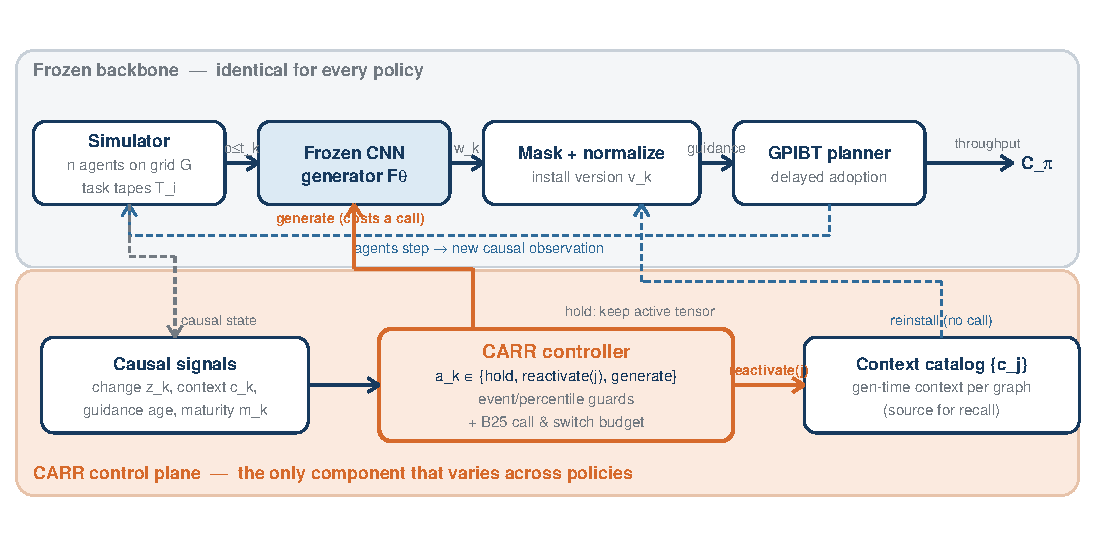
\includegraphics[width=\textwidth]{b_framework.pdf}
\caption{System overview. The convolutional generator $F_\theta$, the GPIBT
planner, the simulator, the maps, and the task tapes form a \emph{frozen
backbone} that is byte-identical for every policy (top band). \carr is a
\emph{control plane} (bottom band) that, at each guidance decision, reads
causally available signals---demand change $z_k$, context $c_k$, guidance age,
and route-adoption maturity $m^{\mathrm{route}}_k$---and selects
\textsc{hold}, \textsc{reactivate}$(j)$, or \textsc{generate} under an explicit
call and switch budget. Only \textsc{generate} invokes $F_\theta$ and spends a
generator call; \textsc{reactivate} reinstalls a cached graph from the context
catalog without a call; \textsc{hold} keeps the active tensor. Installations are
adopted with delay as agents construct new routes.}
\label{fig:framework}
\end{figure*}

\section{Related Work}

\subsection{Multi-agent path finding and its lifelong variants}

Multi-agent path finding (MAPF) computes collision-free paths for many agents
and now has standardized definitions and benchmarks \cite{stern2019benchmarks}.
Optimal solvers such as Conflict-Based Search scale to moderate teams
\cite{sharon2015cbs}, while bounded-suboptimal search \cite{li2021eecbs},
anytime large-neighborhood refinement \cite{li2021mapflns}, and
configuration-space search \cite{okumura2023lacam} push scalability further;
learned decentralized policies instead trade optimality for reactivity
\cite{sartoretti2019primal}. Lifelong or online variants replace one-shot
instances with a continuing task stream: early formulations use
pickup-and-delivery streams and token-passing coordination \cite{ma2017lifelong},
PIBT builds next actions by priority inheritance and backtracking with
finite-time guarantees under specific graph conditions \cite{ijcai2019p76}, and
RHCR repeatedly solves bounded-horizon windows \cite{li2021rhcr}. We do not
empirically compare these solver families; we fix a GPIBT-style downstream
planner so that differences are attributable to guidance publication policy.

\subsection{Global traffic guidance}

Shared directional preferences have progressed from learned direction maps
and user-specified highways \cite{jansen2008direction,cohen2015highways} to
congestion-avoiding guide paths \cite{chen2024traffic}. Guidance Graph
Optimization (GGO) directly optimizes edge weights or a model that produces
them \cite{ijcai2024p0035}; later work extends the representation to mixed edge
directions and weights \cite{zhang2026mixed}. OnlineGGO dynamically generates
guidance from recent traffic and current task distributions and integrates it
with both direct and guide-path planning \cite{zang2025online}. These works
primarily ask what guidance should contain. We keep the learned generator
fixed and ask when its output should be retained, regenerated, or recalled.

\subsection{Adaptive update timing}

Update timing is an established control variable outside LMAPF. Event-triggered
control replaces strictly periodic execution with state-dependent events
\cite{tabuada2007event}; navigation work has studied learned replanning timing
and path-regeneration decisions in dynamic environments
\cite{honda2024when,han2018path}. We borrow the resource-aware motivation, not
their stability or navigation guarantees. Our setting differs in that a shared
guidance artifact influences many agents, adoption is delayed until route
construction, and evidence is evaluated as a paired throughput--call frontier.

\section{Problem Setting and System Semantics}

\subsection{Lifelong routing with fixed guidance generation}

Let $G=(V,E)$ be a directed grid graph and let $n$ agents repeatedly receive
sequential goal-reaching tasks. At each simulator step an agent waits or moves
to an adjacent vertex; vertex conflicts and opposing edge swaps are forbidden.
The planner consults a shared directed-edge guidance tensor while constructing
routes.

A frozen convolutional generator $F_\theta$ maps the causal traffic
observation at decision $k$ to a four-channel raw edge-weight tensor,
\begin{equation}
  w_k=F_\theta(o_{\leq t_k})\in\mathbb{R}^{4\times H_m\times W_m}.
\end{equation}
The environment masks invalid edges and normalizes $w_k$ before the GPIBT
backend consumes it. We vary only the policy that decides whether to hold,
replace, or recall guidance. The checkpoint, planner, simulator, maps, and task
tapes remain fixed.

Each episode contains a 200-step warm-up and a scored horizon of 2,000 steps.
Guidance decisions occur every $D=20$ steps, producing $N=100$ scored windows.
All policies make one mandatory bootstrap call. Of the 99 post-bootstrap
decisions, the focal ceiling is
\begin{equation}
  B_{25}=\lceil0.25(99)\rceil=25.
\end{equation}
For policy $\pi$, let $C_\pi$ be scored task completions, $G_\pi$ fresh
post-bootstrap generator calls, and $S_\pi$ effective post-bootstrap guidance
installations. We study the two-dimensional operating point
$(\mathbb{E}[1+G_\pi],\mathbb{E}[C_\pi])$ and report installations separately.
Generator calls are a pre-specified logical resource unit; they are not a proxy
for a measured wall-clock, energy, or monetary reduction.

\subsection{Policy-independent task tapes}

Completion-driven task generation can confound a throughput comparison: a
faster policy advances its task random-number stream sooner and may receive a
different future workload. We instead materialize complete absolute-release
task tapes before timestep zero. For agent $i$,
\begin{equation}
  \mathcal{T}_i=((g_{i,0},r_{i,0}),\ldots,(g_{i,L_i-1},r_{i,L_i-1})),
\end{equation}
where $g_{i,j}$ is a goal and $r_{i,j}$ its absolute release time. Starts,
goals, releases, and identifiers are identical across paired policies and are
verified by independent fingerprints. We evaluate stationary, abrupt, and
recurrent endpoint distributions; recurrent demand follows an
$A\!\rightarrow\!B\!\rightarrow\!A\!\rightarrow\!B$ sequence. Phase metadata
and unreleased tape suffixes are never controller inputs.

\subsection{Generation, installation, and delayed adoption}

A \emph{generation ID} names one immutable output of $F_\theta$. An
\emph{installation version} increments whenever a fresh or historical graph
becomes active. Reactivating a graph changes its installation version but not
its generation ID. Holding still advances the simulator using a defensive copy
of the cached raw tensor.

An installation affects an agent only when the planner constructs a route.
Agents already following routes may therefore retain older versions. For
active version $v_k$, we measure route-adoption maturity as
\begin{equation}
 m_k^{\mathrm{route}}=
 \frac{\#\{\text{active agents whose latest route uses }v_k\}}
      {\#\{\text{active agents}\}}.
\end{equation}
This distinction prevents the controller from treating publication as an
instantaneous fleet-wide state change.

\section{Context-Aware Refresh and Recall}

The paper name \carr corresponds exactly to the evaluated implementation
\texttt{context\_memory\_B25}; no post-evaluation behavior change is hidden by
the renaming. Its action set is
\begin{equation}
 a_k\in\{\textsc{hold},\textsc{reactivate}(j),\textsc{generate}\}.
\end{equation}

\subsection{Causal change signal}

Goals released in the current trace window are binned into a $4\times4$
spatial histogram with a 0.5 pseudocount per bin. Let $p_k^f$ average the two
most recent non-missing windows and let $p_k^s$ average up to six preceding
non-missing windows. The normalized change score is
\begin{equation}
 z_k=\operatorname{JS}(p_k^f,p_k^s)/\log 2\in[0,1],
\end{equation}
and is zero when either side is unavailable. Thresholds are computed from
past scores before appending $z_k$, so future tasks, latent phases, and future
rewards cannot influence an earlier action.

\subsection{Context catalog and recall}

For each generated graph $j$, \carr stores the causal $4\times4$ distribution
$c_j$ of active goals at generation time. With current context $c_k$,
\begin{equation}
 d_{k,j}=\operatorname{JS}(c_k,c_j)/\log 2.
\end{equation}
Let $a$ be the active generation and $j^*$ the nearest inactive catalog item.
Recall is available only if
\begin{equation}
 d_{k,j^*}\leq0.05
 \quad\text{and}\quad
 d_{k,a}-d_{k,j^*}\geq0.02.
\end{equation}
The controller first proposes an available historical match; otherwise it
generates when maintenance is due, holds if active context still matches, or
proposes a fresh generation. Maintenance is due after 25 guidance-age windows
when $z_k\leq0.20$.

\subsection{Execution guards and budgets}

A proposed switch is executed only if maintenance is due or the event signal
is at least 0.10 and strictly above the historical 75th percentile after four
history observations. It must also satisfy
$m_k^{\mathrm{route}}\geq0.5$, a six-window minimum gap, at least three
remaining effect windows, and the unspent cap. Both fresh generations and
effective switches are capped at $B_{25}$. A reactivation consumes a switch
token but no generator token; a fresh generation consumes both. There is no
catch-up or forced budget fill.

This is a ceiling, not a six-call hard budget. \carr's call count is an outcome
and reaches 10 in the confirmation matrix. Comparisons with G4/G5 schedules
therefore bracket its observed mean; they are not per-run call-matched trials.
Algorithm~\ref{alg:carr} consolidates one decision window: signal computation,
proposal, execution guard, and budgeted application.

\begin{algorithm}[t]
\caption{\carr decision at guidance window $k$ (\texttt{context\_memory\_B25}).}
\label{alg:carr}
\begin{algorithmic}[1]
\Require active generation $a$; context catalog $\{c_j\}$; event-score history
  $H$; guidance age; call/switch budgets
\State $z_k \gets \operatorname{JS}(p^f_k,p^s_k)/\log 2$
  \Comment{causal demand-change score}
\State $j^\ast \gets \arg\min_{j\,\text{inactive}} d_{k,j}$
\State $\mathit{recall} \gets (d_{k,j^\ast}\!\le\!0.05)\wedge
  (d_{k,a}\!-\!d_{k,j^\ast}\!\ge\!0.02)$
\State $\mathit{due} \gets (\text{age}\!\ge\!25)\wedge(z_k\!\le\!0.20)$
  \Comment{maintenance due}
\If{$\mathit{recall}$}
  \State $\mathit{prop} \gets \textsc{reactivate}(j^\ast)$
\ElsIf{$\mathit{due}$}
  \State $\mathit{prop} \gets \textsc{generate}$
\ElsIf{active context still matches}
  \State $\mathit{prop} \gets \textsc{hold}$
\Else
  \State $\mathit{prop} \gets \textsc{generate}$
\EndIf
\State $\mathit{trig} \gets \mathit{due} \vee
  (z_k\!\ge\!0.10 \wedge z_k\!>\!Q_{75}(H) \wedge |H|\!\ge\!4)$
\State $\mathit{ok} \gets \mathit{trig} \wedge (m^{\mathrm{route}}_k\!\ge\!0.5)
  \wedge (\text{gap}\!\ge\!6) \wedge (\text{windows left}\!\ge\!3)
  \wedge \text{budget left}$
\If{$\mathit{prop}\in\{\textsc{generate},\textsc{reactivate}\}$ and
    $\neg\,\mathit{ok}$}
  \State $a_k \gets \textsc{hold}$
\Else
  \State $a_k \gets \mathit{prop}$
\EndIf
\If{$a_k = \textsc{generate}$}
  \State call $F_\theta$; install fresh graph; spend call $+$ switch token
\ElsIf{$a_k = \textsc{reactivate}(j^\ast)$}
  \State reinstall $c_{j^\ast}$; spend switch token only
\Else
  \State advance simulator with cached tensor
\EndIf
\State append $z_k$ to $H$
\end{algorithmic}
\end{algorithm}

\section{Experimental Design}

\subsection{Scenarios and workloads}

All arms use the same frozen 3,084-parameter OnlineGGO-style CNN checkpoint
and pinned GPIBT simulator. Table~\ref{tab:scenarios} crosses two warehouse
maps with two densities. Each scenario is run with stationary, abrupt, and
recurrent task streams.

\begin{table}[t]
\caption{Frozen scenarios.}
\label{tab:scenarios}
\centering
\small
\begin{tabular}{lcr}
\toprule
Scenario & Map family & Agents \\
\midrule
\texttt{narrow\_r020}  & narrow  & 218 \\
\texttt{narrow\_r035}  & narrow  & 382 \\
\texttt{regular\_r020} & regular & 255 \\
\texttt{regular\_r035} & regular & 447 \\
\bottomrule
\end{tabular}
\end{table}

Forty root clusters were fixed before execution. The complete matrix contains
$8$ policies $\times40$ roots $\times4$ scenarios $\times3$ workloads = 3{,}840
runs. Every policy has 480 paired cells, but the root---not a cell, window,
task, or agent---is the independent unit.

Before Experiment~B, a 960-run, ten-root A2 experiment on the same backbone
failed its pre-specified 1\% non-inferiority test: its mean effect was
$-0.4009\%$, with a 95\% interval of [$-1.0834\%$, $0.2584\%$] and shifted
one-sided $p=.06836$. Simulations that resampled centered A2 root residuals
informed B's 40-root sample-size choice, but those simulations were design
calculations rather than B evidence. B uses forty fresh roots disjoint from A2;
the studies are reported separately and are never pooled.

\subsection{Publication policies}

Table~\ref{tab:policies} lists the frozen controller family. \norecall maps to
\texttt{context\_no\_reactivation\_B25} and changes only recall availability.
\exactdense provides the high-call reference.

\begin{table*}[t]
\caption{Evaluated publication policies. Counts include the mandatory
bootstrap call where stated.}
\label{tab:policies}
\centering
\small
\begin{tabular}{lll}
\toprule
Paper name & Frozen implementation & Publication contract \\
\midrule
\bbootstrap & \texttt{bootstrap\_only} & Bootstrap once, then hold \\
\exactfour & \texttt{exact\_even\_G4} & Bootstrap + 4 even calls (5 total) \\
\exactfive & \texttt{exact\_even\_G5} & Bootstrap + 5 even calls (6 total) \\
\randomfive & \texttt{random\_G5} & Bootstrap + 5 root-keyed random calls \\
\jsfive & \texttt{js\_cap\_G5} & Causal JS trigger, at most 5 post calls \\
\norecall & \texttt{context\_no\_reactivation\_B25} & \carr logic without historical recall \\
\carr & \texttt{context\_memory\_B25} & Hold/reactivate/generate under B25 ceilings \\
\exactdense & \texttt{exact\_even\_B25} & Bootstrap + 25 even calls (26 total) \\
\bottomrule
\end{tabular}
\end{table*}

\subsection{Frozen inference and integrity}

For focal policy $A$ and comparator $B$, the pre-specified root effect averages
the 12 scenario--workload cells equally:
\begin{equation}
 d_i(A,B)=\frac{1}{12}\sum_{c=1}^{12}
 \frac{C_{A,i,c}-C_{B,i,c}}{C_{B,i,c}}.
\end{equation}
We report the mean of forty root effects, root win/tie/loss counts, and a
10,000-sample whole-root percentile-bootstrap 95\% interval
\cite{efron1993bootstrap}. Superiority uses one-sided exact paired sign-flip
(permutation) tests \cite{good2005permutation}---computed exactly over the
$2^{40}\approx1.1\times10^{12}$ root sign assignments by a meet-in-the-middle
enumeration---with Holm step-down correction \cite{holm1979} over six frozen
contrasts. The separate test against \exactdense uses a $-1\%$ non-inferiority
margin \cite{wellek2010noninferiority} and requires all three frozen
conditions: mean effect at least $-0.5\%$, interval lower bound strictly above
$-1\%$, and shifted one-sided exact $p<.05$.

Each arm ran in a fresh process. Append-only ledgers bind the arm, process
instance, run UUID, paired-input fingerprints, safety state, and output hash.
The audit requires the exact Cartesian product, one start and completion per
arm, zero hidden retries or deletions, matched exogenous inputs, valid budget
schedules, and zero collisions, swaps, invalid moves, or planner timeouts.
The controller definitions, matrix, estimands, inference, stopping
rule, and audit gates were internally pre-specified and frozen before
execution, and the forty roots were fixed before any fresh-root run; we do not
describe this internal freeze as public preregistration.

\section{Results}

\subsection{Integrity and primary non-inferiority result}

All 3{,}840 runs passed the integrity audit. The pre-specified primary B
objective was not met. \carr completes 49.29 fewer tasks than \exactdense on
the grand mean. Its root-level relative effect is $-0.8006\%$, with a 95\%
interval of [$-1.1935\%$, $-0.3966\%$] and a shifted exact one-sided
$p=.1693$. All three pre-specified conditions fail: the mean effect is below
$-0.5\%$, the interval lower bound is not strictly above $-1\%$, and the
shifted test does not pass $.05$. The frozen 1\% non-inferiority criterion
therefore fails. The interval lies entirely below zero, indicating a measurable
throughput deficit on this benchmark; it does not establish that \carr
preserves throughput within 1\% of dense refresh.

Table~\ref{tab:decomp} reports the pre-specified decomposition. The deficit is
concentrated on the dense regular map: by workload it grows from $-0.31\%$ under
stationary demand to $-1.33\%$ under abrupt shifts, and by scenario from
$-0.37\%$ in \texttt{narrow\_r035} to $-1.71\%$ in \texttt{regular\_r035}. These
decompositions illustrate heterogeneity but do not replace the failed aggregate
test.

\begin{table}[t]
\caption{Pre-specified decomposition of the primary non-inferiority effect
(\carr minus \exactdense). Negative values favor dense refresh; ``Effect'' is
the mean relative throughput difference over the constituent root--scenario
cells.}
\label{tab:decomp}
\centering
\small
\begin{tabular}{lrrr}
\toprule
Subgroup & Cells & Task $\Delta$ & Effect \\
\midrule
\multicolumn{4}{l}{\emph{By map}}\\
\quad narrow  & 240 & $-24.07$ & $-0.41\%$ \\
\quad regular & 240 & $-74.50$ & $-1.19\%$ \\
\addlinespace
\multicolumn{4}{l}{\emph{By scenario}}\\
\quad \texttt{narrow\_r020}  & 120 & $-17.83$  & $-0.44\%$ \\
\quad \texttt{narrow\_r035}  & 120 & $-30.32$  & $-0.37\%$ \\
\quad \texttt{regular\_r020} & 120 & $-30.96$  & $-0.68\%$ \\
\quad \texttt{regular\_r035} & 120 & $-118.04$ & $-1.71\%$ \\
\addlinespace
\multicolumn{4}{l}{\emph{By workload}}\\
\quad stationary & 160 & $-20.61$ & $-0.31\%$ \\
\quad recurrent  & 160 & $-49.57$ & $-0.76\%$ \\
\quad abrupt     & 160 & $-77.68$ & $-1.33\%$ \\
\midrule
Overall & 480 & $-49.29$ & $-0.80\%$ \\
\bottomrule
\end{tabular}
\end{table}

\subsection{Throughput and generator calls}

The pre-specified secondary analyses characterize the operating point after
the failed primary test. Table~\ref{tab:operating-points} reports mean
throughput and generator calls, and Figure~\ref{fig:pareto} plots the
corresponding operating points. \carr completes 4{,}539.62 tasks with 5.46
calls on average. Its empirical call distribution is sparse but variable:
median 5, 90th percentile 8, and maximum 10.

\begin{figure*}[t]
\centering
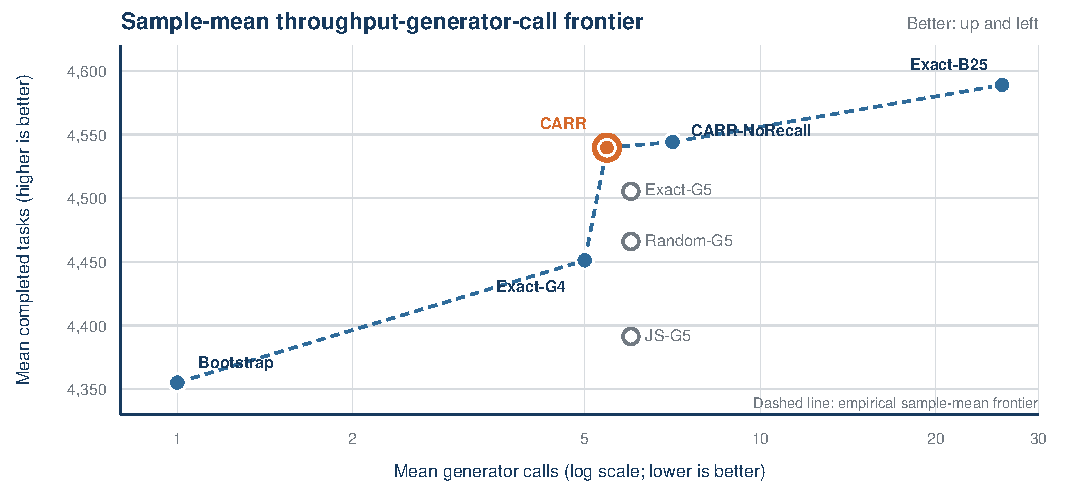
\includegraphics[width=0.88\textwidth]{b_pareto_frontier.pdf}
\caption{Sample-mean throughput--generator-call operating points. The dashed
line joins the empirical mean frontier; it is not an uncertainty-aware
dominance claim. \carr is highlighted in orange.}
\label{fig:pareto}
\end{figure*}

\begin{table*}[t]
\caption{Sample-mean operating points. Frontier membership concerns the two
point estimates (mean tasks, mean calls), not statistical dominance.}
\label{tab:operating-points}
\centering
\small
\begin{tabular}{lrrrrrrc}
\toprule
Policy & Tasks & Calls mean & Median & P90 & Max & Reactivations & Frontier \\
\midrule
\bbootstrap & 4355.08 & 1.00 & 1.0 & 1 & 1 & 0.00 & yes \\
\exactfour & 4451.10 & 5.00 & 5.0 & 5 & 5 & 0.00 & yes \\
\exactfive & 4505.35 & 6.00 & 6.0 & 6 & 6 & 0.00 & no \\
\randomfive & 4465.94 & 6.00 & 6.0 & 6 & 6 & 0.00 & no \\
\jsfive & 4391.32 & 6.00 & 6.0 & 6 & 6 & 0.00 & no \\
\norecall & 4544.06 & 7.07 & 7.0 & 10 & 13 & 0.00 & yes \\
\carr & 4539.62 & 5.46 & 5.0 & 8 & 10 & 1.74 & yes \\
\exactdense & 4588.90 & 26.00 & 26.0 & 26 & 26 & 0.00 & yes \\
\bottomrule
\end{tabular}
\end{table*}

The sample-mean frontier is \bbootstrap, \exactfour, \carr, \norecall, and
\exactdense. \carr point-dominates the three six-call G5 controls on sample
means, but this does not imply pairwise statistical superiority. Relative to
\exactdense, calls decrease from 26 to 5.46, a descriptive reduction of
79.01\%. No corresponding runtime reduction is claimed.

\subsection{Which secondary sparse comparisons are supported?}

Table~\ref{tab:contrasts} and Figure~\ref{fig:forest} report the six frozen
superiority contrasts. After Holm correction, \carr is significantly superior
to all five frozen low-call comparators---\bbootstrap, \exactfour, \exactfive,
\randomfive, and \jsfive---including the strongest fixed six-call periodic
schedule. It is not superior to its own \norecall ablation, whose interval
crosses zero (Holm $p=.925$); a confidence interval crossing zero is not
evidence of equality.

\begin{figure*}[t]
\centering
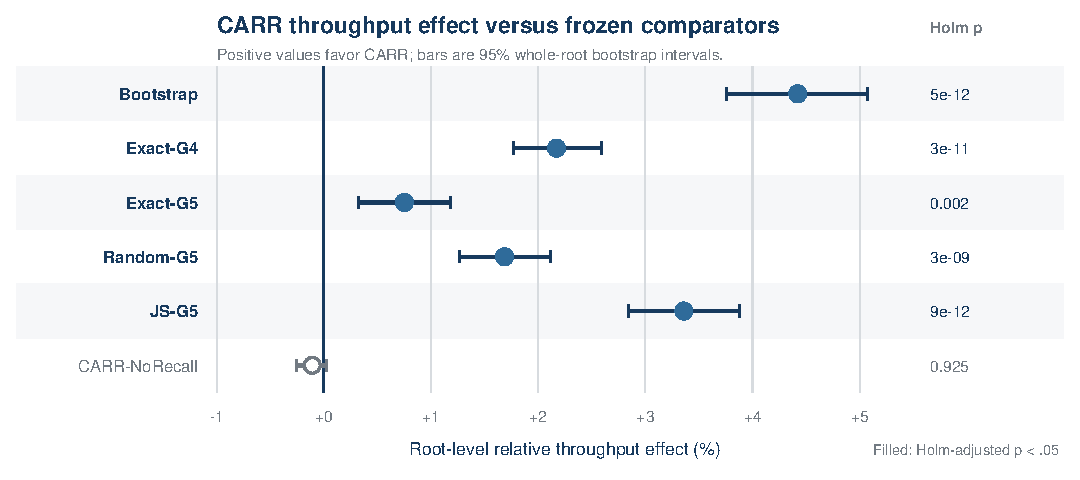
\includegraphics[width=0.88\textwidth]{b_superiority_forest.pdf}
\caption{Frozen root-level superiority contrasts for \carr. Filled points
remain significant after Holm correction; a confidence interval crossing
zero is not evidence of equality.}
\label{fig:forest}
\end{figure*}

\begin{table*}[t]
\caption{Root-level effects of \carr minus each comparator. Positive values
favor \carr. Intervals are whole-root bootstrap intervals.}
\label{tab:contrasts}
\centering
\small
\begin{tabular}{lrrrrrr}
\toprule
Comparator & Task $\Delta$ & Mean effect & 95\% CI & W/T/L & Raw $p$ & Holm $p$ \\
\midrule
\bbootstrap & +184.54 & +4.42\% & [3.75, 5.07]\% & 40/0/0 & $9.1{\times}10^{-13}$ & $5.5{\times}10^{-12}$ \\
\exactfour & +88.52 & +2.17\% & [1.77, 2.59]\% & 37/0/3 & $7.3{\times}10^{-12}$ & $2.9{\times}10^{-11}$ \\
\exactfive & +34.26 & +0.75\% & [0.32, 1.18]\% & 28/0/12 & $7.7{\times}10^{-4}$ & $1.5{\times}10^{-3}$ \\
\randomfive & +73.68 & +1.69\% & [1.27, 2.11]\% & 36/0/4 & $1.1{\times}10^{-9}$ & $3.4{\times}10^{-9}$ \\
\jsfive & +148.30 & +3.36\% & [2.85, 3.87]\% & 39/0/1 & $1.8{\times}10^{-12}$ & $9.1{\times}10^{-12}$ \\
\norecall & $-4.44$ & $-0.11\%$ & [$-0.26$, 0.03]\% & 18/0/22 & $.925$ & $.925$ \\
\bottomrule
\end{tabular}
\end{table*}

\subsection{What does historical recall contribute?}

Against \norecall, \carr's throughput effect is $-0.108\%$ (95\% CI
[$-0.257\%$, $0.029\%$]; Holm $p=.925$). Thus the experiment detects no
throughput benefit from recall. The observed mean total-call count falls from
7.07 to 5.46 (22.8\%), and post-bootstrap fresh generations fall from 6.07 to
4.46 (26.6\%), while effective switches rise slightly from 6.07 to 6.20 because
1.74 historical graphs are reactivated on average. These call differences are
descriptive; no call-difference significance test was pre-specified. The
supported mechanism statement is therefore narrow: recall substitutes for some
fresh generations, not that it improves throughput.

\section{Discussion and Limitations}

\paragraph{When should guidance be refreshed?}
The results favor neither always holding nor refreshing at every opportunity.
Relative to bootstrap-only reuse, context-aware publication yields +4.42\%
throughput; relative to a 26-call schedule, it spends 79.01\% fewer calls but
carries a measurable throughput deficit whose 95\% interval lies entirely
below zero yet extends past the $-1\%$ margin. Unlike the ten-root A2 study,
the pre-specified secondary comparison with the fixed six-call even schedule
now favors \carr after correction. The practical answer is therefore an
operating curve rather than a universally best trigger: \carr is useful when
generator calls are the constrained unit, but dense refresh remains the
highest-throughput sample mean.

\paragraph{Coordination-system relevance.}
The unit controlled by \carr is a shared artifact that many agents adopt at
different route-construction times. Explicit installation versions and route
maturity make this delayed adoption auditable. This control-plane view is
applicable to distributed agent systems in which an expensive shared policy,
plan, or coordination signal is recomputed less frequently than local actions.
Our evidence, however, is specific to the evaluated routing backbone.

\paragraph{External validity.}
The study fixes one small CNN checkpoint, one GPIBT-style backbone, two related
warehouse maps, two densities, three synthetic workload families, and forty
independent root clusters. It neither compares against external LMAPF systems
nor establishes global SOTA. Generalization to other maps, generators,
planners, or task models remains open.

\paragraph{Resource interpretation.}
Generator calls are logical counts. We did not obtain valid serial timing,
GPU-time, energy, or financial-cost measurements. Concurrent experiment
execution cannot be repurposed as timing evidence, so call reduction must not
be read as proportional wall-clock acceleration.

\paragraph{Statistical and Pareto uncertainty.}
There are forty independent root clusters; 3{,}840 runs are not 3{,}840
independent replicates. Exact sign-flip inference is computed over
$2^{40}\approx1.1\times10^{12}$ root sign assignments by meet-in-the-middle.
The larger sample tightens the non-inferiority interval relative to A2, but the
B interval still extends below the $-1\%$ margin while lying entirely below
zero; increased precision does not establish non-inferiority. Frontier
membership uses grand sample means and is not an uncertainty-aware
Pareto-dominance test.

\paragraph{Budget comparability and mechanism identification.}
\carr is sparse on average but is not a hard G5 method; 24.0\% of its runs
exceed six calls. Moreover, the no-recall ablation has slightly higher mean
throughput. The evidence cannot attribute the operating point to memory alone.

\paragraph{Analysis provenance.}
The controller matrix, estimands, tests, and stopping rules were frozen
before execution, and the forty roots were fixed before any fresh-root run. The
emphasis on a Pareto operating point is a transparent post-validation narrowing
after a stronger near-dense claim was not supported. We therefore report the
failed non-inferiority result in the abstract, results, and conclusion rather
than presenting the descriptive frontier as the original confirmatory claim.

\section{Conclusion}

We studied when a fixed OnlineGGO-style guidance generator should be invoked
within a GPIBT lifelong-routing backbone. Across 3{,}840 audited paired runs
over forty independent roots, the primary 1\% non-inferiority objective is not
met: \carr has a $-0.80\%$ mean throughput effect relative to 26-call dense
refresh (95\% CI [$-1.19\%$, $-0.40\%$]). In the pre-specified secondary
analyses, \carr uses 5.46 calls on average---79.01\% fewer than dense
refresh---significantly outperforms all five frozen low-call comparators, and
lies on the sample-mean throughput--call frontier. Historical recall replaces
some fresh generations without a detected throughput benefit. The resulting
contribution is a bounded resource--throughput evaluation and an auditable
low-call operating point, not a lossless replacement or global LMAPF SOTA.

\bibliographystyle{ACM-Reference-Format}
\bibliography{references}

\appendix

\section{Execution Audit Summary}

\begin{table}[h]
\caption{Frozen Experiment~B integrity audit.}
\centering
\small
\begin{tabular}{lr}
\toprule
Audit item & Result \\
\midrule
Required runs & 3{,}840/3{,}840 \\
Started/completed attempts & 3{,}840/3{,}840 \\
Unique process instances & 3{,}840 \\
Unique canonical run UUIDs & 3{,}840 \\
Unique bare PIDs (non-gating) & 3{,}829 \\
Method failures/retries & 0 \\
Planner timeouts & 0 \\
Selective/timeout deletions & 0 \\
Safety, pairing, budgets & all pass \\
\bottomrule
\end{tabular}
\end{table}

Experiment~B used forty fresh roots disjoint from the prior ten-root A2
experiment. A2 informed sample-size planning but contributes no root, estimate,
interval, or p-value to B. Earlier in the program, one launcher execution was
discarded effect-blind after it treated legal operating-system PID reuse as
duplicate process identity; no outcome or method ranking from it entered
estimation or interpretation. In B, 11 legal bare-PID reuses yielded 3{,}829
distinct PIDs, while all 3{,}840 host--PID--start-time process instances and run
UUIDs remained unique; bare PID alone was therefore not an integrity gate.

\section{Reproducibility Provenance}

Before execution, the Experiment~B protocol, configuration, implementation
freeze, environment attestation, and preflight evidence were sealed by
SHA-256. After execution, the integrity report, machine-readable analysis,
human-readable report, and complete archive were separately content-hashed.
The final analysis artifact is
\texttt{reports/same\_call\_confirmation\_b\_analysis.json} with digest
\texttt{\seqsplit{cceab3d62390d6a1acd1c5ee3e78ff2048851a20c448796f968f212db0fb428b}};
the complete run archive has digest
\texttt{\seqsplit{6acf741f7ac460458558f1892030b46072fa438e59f639196fee394a5d3658e0}}.
The anonymized artifact will include the complete manifests, source hashes,
ledger checks, analysis and figure-generation scripts, and controller-name
mapping. Its machine-readable analysis also reports all forty root effects,
their median, map/workload/scenario decompositions, and leave-one-root-out
means committed by the frozen protocol.

\end{document}
